\section{Algoritmo de watershed}
\label{chap:marco}

El algoritmo propuesto en este trabajo se basa en la implementación del algoritmo de Vincent y Soille~\cite{VincentSoille}, el cual propone un enfoque de crecimiento de regiones a partir de los mínimos locales. A continuación se muestra un ejemplo gráfico para mejorar el entendimiento. Se hace una analogía con la geografía como se muestra en la Figura \ref{img:relieve}(a). Cada uno de los relieves topográficos de la imagen son inundados con agua, donde las líneas watershed son las divisorias de distintos depósitos de agua~\cite{parwashed}. Las entradas del algoritmo son la gradiente morfológica de la imagen y los marcadores. La transformación watershed puede ser clasificada bajo el enfoque de segmentación basado en regiones. 

El algoritmo de watershed en escala de grises descrito por Vincent y Soille~\cite{VincentSoille} realiza una inundación por niveles, desde el mínimo hasta el máximo nivel de intensidad de los píxeles de la imagen. En las Figuras \ref{img:relieve}(b),(c) y (d) se muestra como se van inundando los niveles. Las zonas de baja intensidad se conocen como vasijas (basins en Inglés), por donde fluirá el agua e inundará toda la imagen; es decir, el agua fluirá en cada una de las vasijas identificadas a partir de los mínimos de la imagen. El proceso de inundación continúa hasta que las aguas de cuencas o vasijas contiguas se unan, formando líneas de unión que representarán las fronteras de regiones homogéneas, y constituyen el resultado de la segmentación~\cite{parwashed}, como se muestra en la Figura \ref{img:relieve}(e). El crecimiento de regiones se inicia a partir de marcadores obtenidos por la selección de todos los mínimos del gradiente, lo que podría producir una segmentación no deseada. En la Figura \ref{img:relieve}(e) se muestra como el objeto segmentado fue dividido en el medio, produciendo un resultado no deseado.
\begin{figure}[H]
\centering
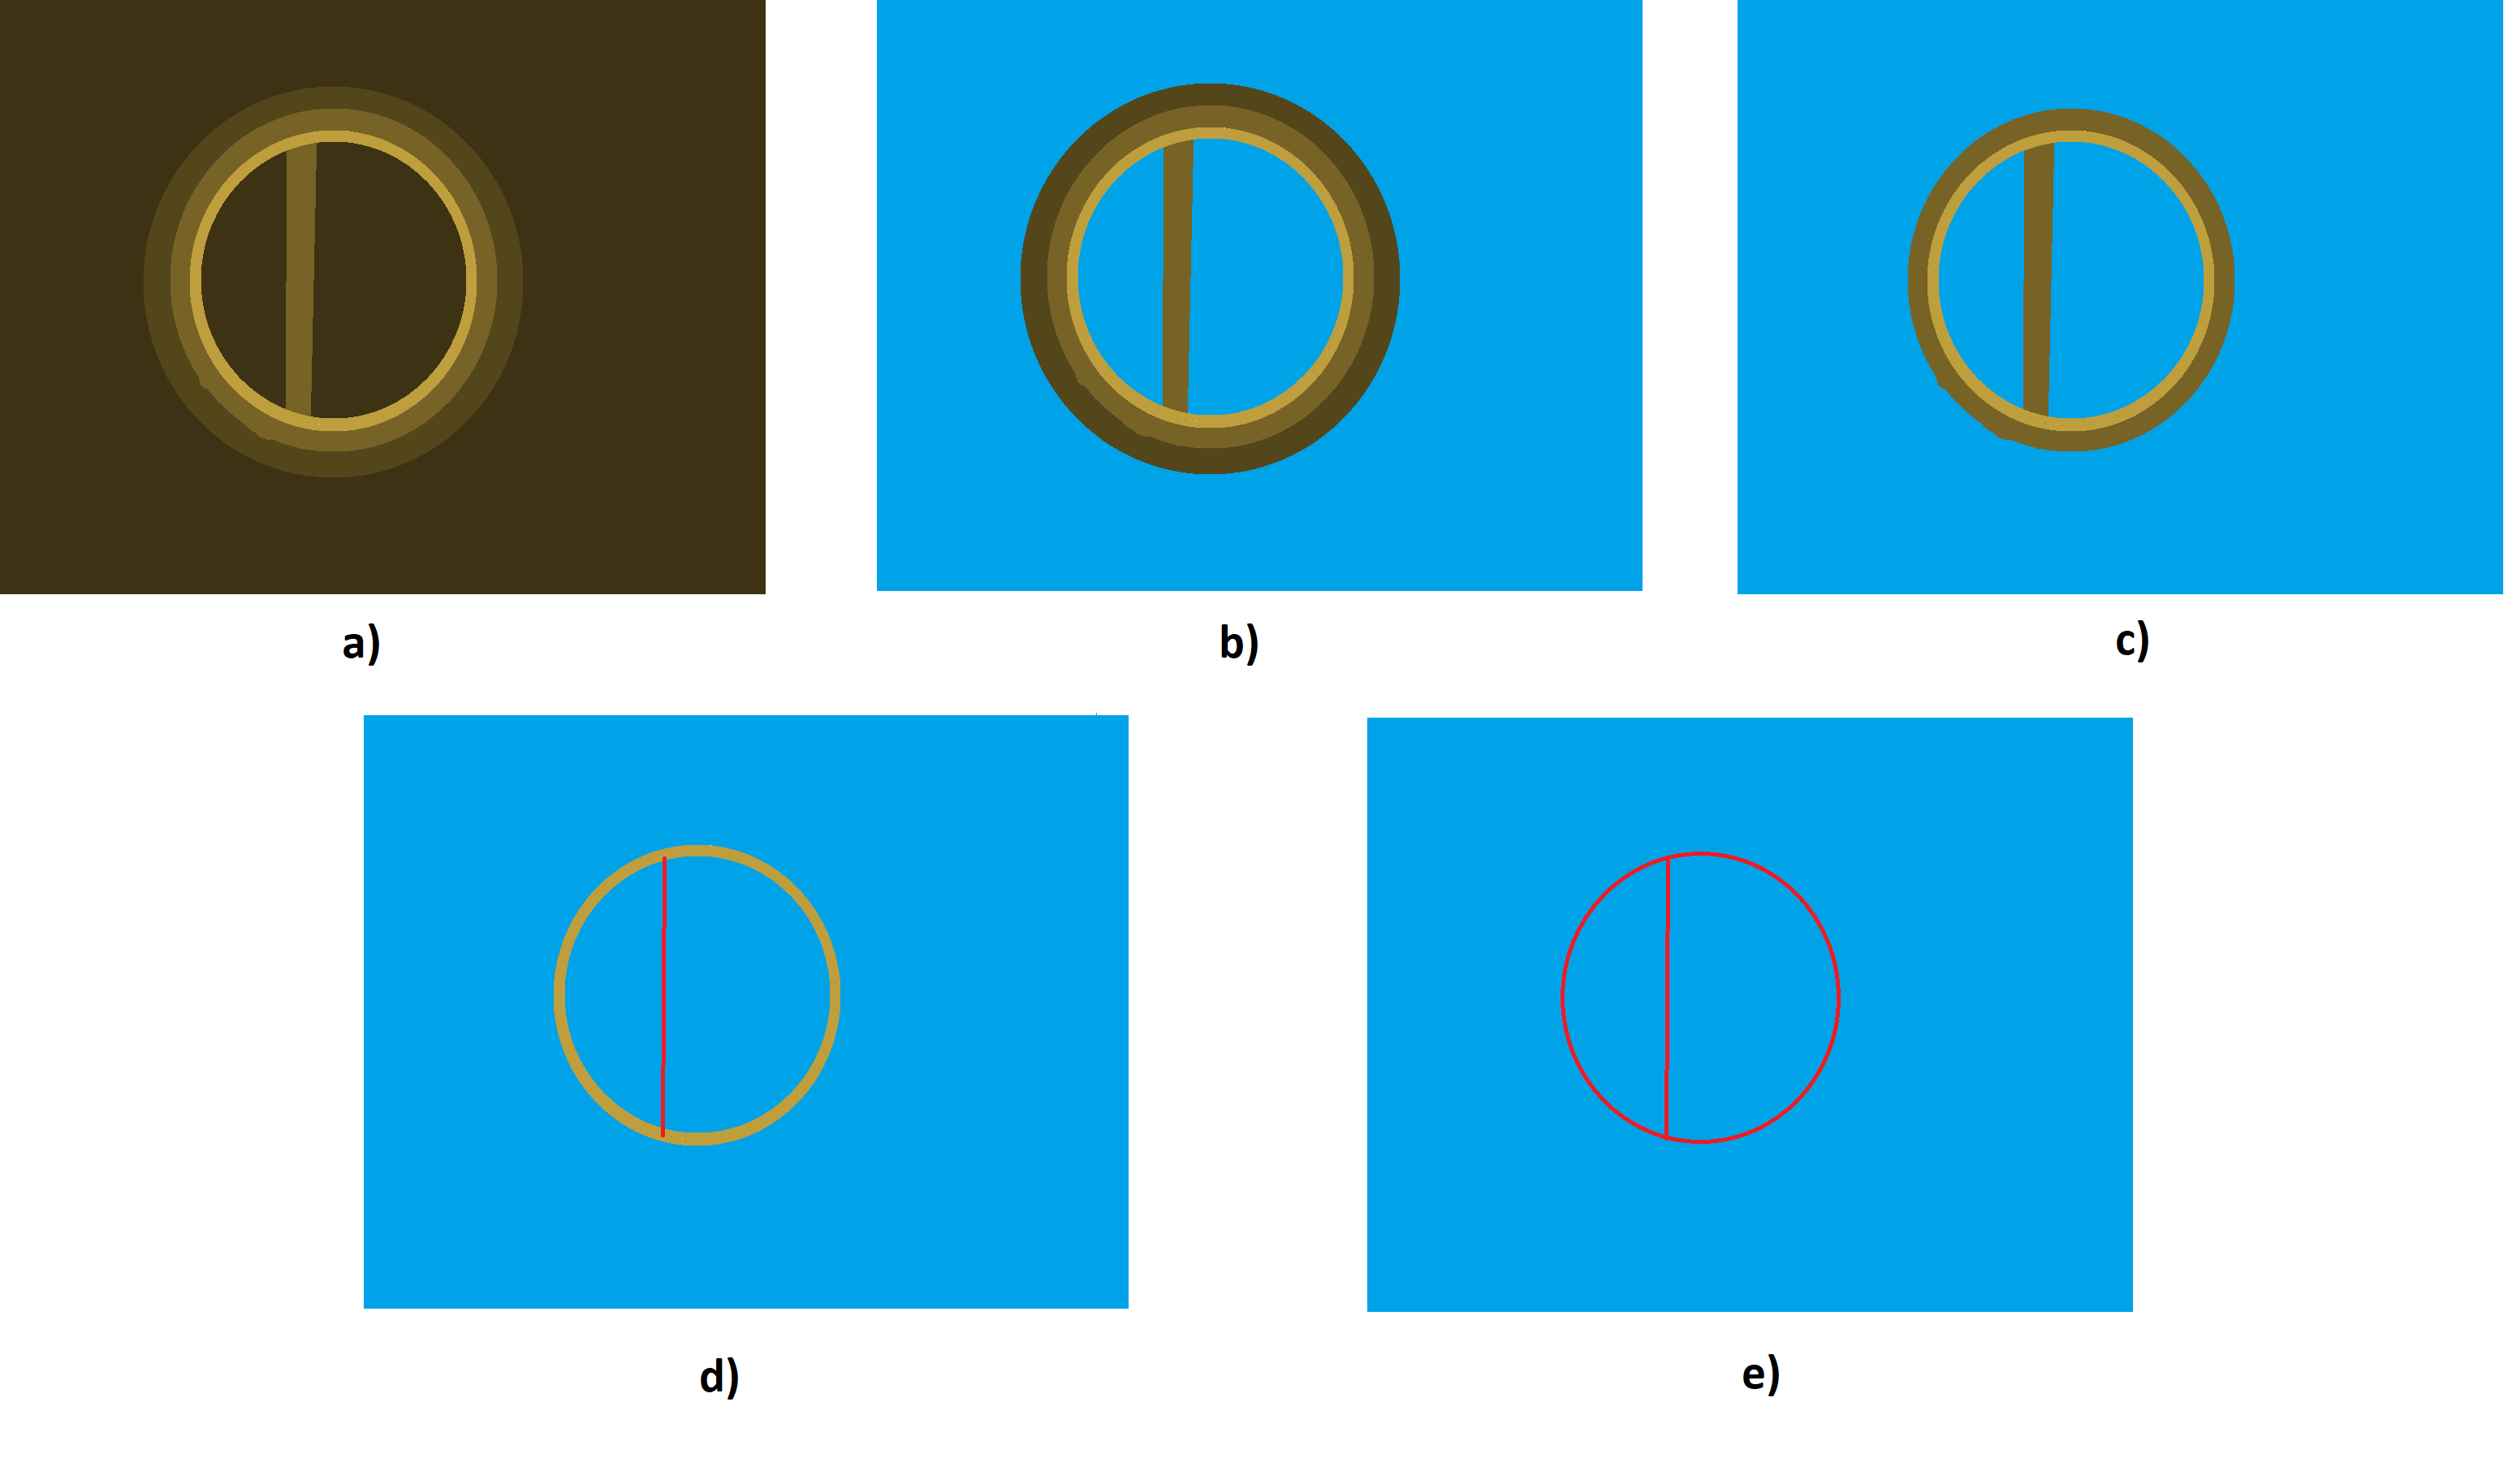
\includegraphics[width=150mm]{./imagenes/sin_marcadores.png}
\caption{Proceso de inundación con resultados no deseados}
\label{img:relieve}
\end{figure}

Al momento de la inundación, se tiene en cuenta una relación de orden dual entre los píxeles a ser inundados. La relación dual se entiende como la dependencia que existe entre dos criterios de ordenamiento, el orden de llegada a la cola y la altura de los píxeles. Un píxel de menor altura se debe inundar primero, así también los vecinos que se encuentren en una misma altura deben ser inundados antes de seguir con el orden anterior. Un algoritmo que simule la inundación tiene que poder reproducir la relación de orden dual, que naturalmente se obtiene con el uso de una cola de prioridad. Una cola de prioridad permite almacenar puntos en cualquier orden y devolverlos en el orden de la inundación.

El proceso de watershed para imágenes cromáticas puede afrontarse desde diversos enfoques. El empleo de información cromática en el proceso de watershed es posible por ejemplo, calculando el watershed en cada una de las señales cromáticas y combinar después los resultados~\cite{Saarinen}. Otra posibilidad es calcular el watershed directamente sobre la imagen a color~\cite{Meyer}.

La transformación watershed permite calcular los contornos más relevantes de la imagen, pudiendo así seleccionar los resultados deseados~\cite{Meyer}. En algunos casos donde las imágenes en escala de grises no presentan grandes variaciones de intensidad entre diferentes cuerpos, podría obtenerse una segmentación no esperada. Considere la misma imagen pero esta vez a color, podría tener los mismos niveles de intensidad pero en diferentes canales, en cuyo caso visualmente se distingue de manera fácil la diferencia entre diferentes cuerpos. El color es una propiedad distinguible entre diferentes regiones de una imagen por lo cual una segmentación a color puede tener mejores resultados que una en escala de grises~\cite{Lezoray}.

\subsection{Marcadores}
Generalmente los puntos iniciales de la inundación son mínimos locales y los marcadores denotan la cantidad de regiones a ser obtenidas luego del proceso de segmentación. En algunas imágenes se tiene la presencia de un gran número de mínimos locales, produciéndose sobre-segmentación en pequeñas regiones. Muchas de las regiones generadas no son importantes dentro de la imagen, o no representan objetos existentes en la imagen original.

La sobre-segmentación se puede disminuir utilizando métodos de mejora como filtros morfológicos. Además de ellos se podrían aplicar otras formas para evitar la sobre-segmentación, como es la selección de marcadores. Seleccionar marcadores en la imagen resuelve dicho problema iniciando el proceso de inundación desde los píxeles marcados, que representan los objetos deseados a segmentar en la imagen~\cite{Yang}. En este trabajo los marcadores fueron seleccionados manualmente.

La imagen que se muestra en la Figura \ref{img:relieve1}(a) contiene un objeto circular que se desea segmentar. Para evitar una segmentación no deseada fueron seleccionados dos marcadores, uno dentro del objeto deseado y otro en el fondo de la imagen, como se muestra en la Figura \ref{img:relieve1}(b). Posteriormente se inicia el proceso de inundación a partir de los marcadores como se muestra en las Figuras \ref{img:relieve1}(c), (d) y (e). En la Figura \ref{img:relieve1}(f) se muestra el resultado de la segmentación del objeto deseado.


\begin{figure}[H]
\centering
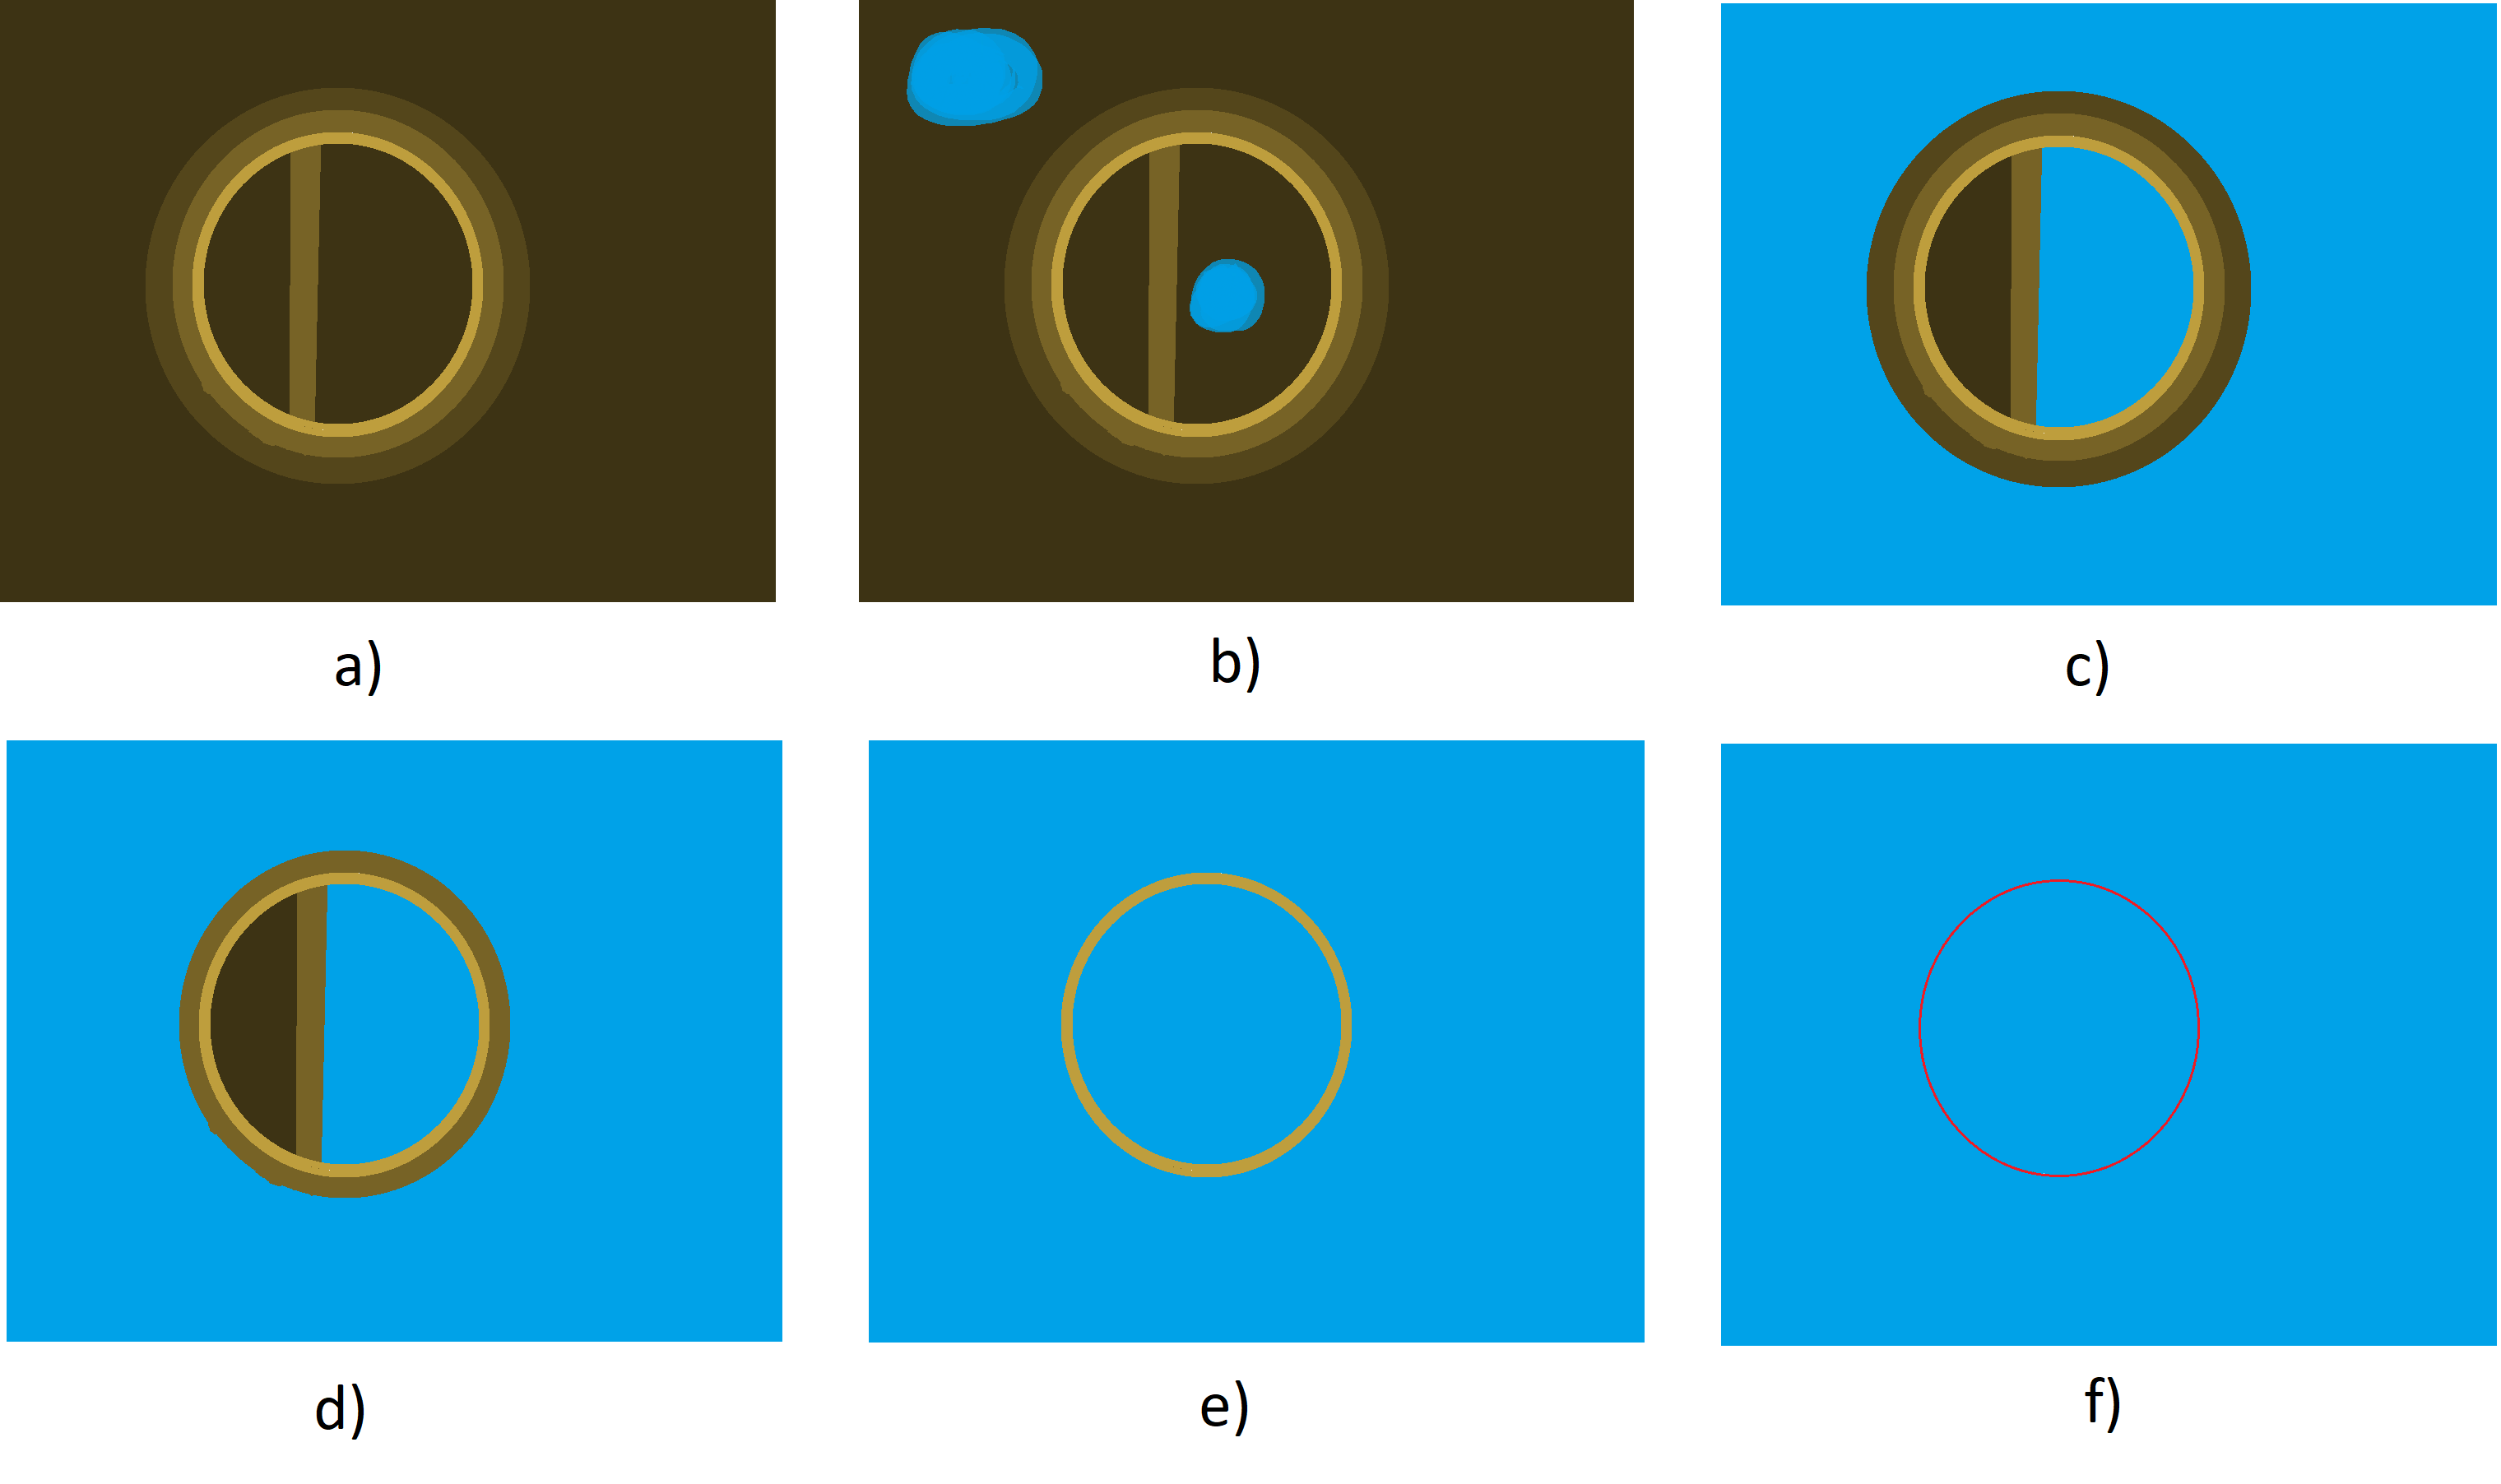
\includegraphics[width=140mm]{./imagenes/con_marcadores.png}
\caption{Proceso de inundación con marcadores del objeto deseado}
\label{img:relieve1}
\end{figure}

